\documentclass{article}
\usepackage[a4paper, margin=1in]{geometry}
\usepackage[T1]{fontenc}
\usepackage[utf8]{inputenc}
\usepackage{lmodern}
\usepackage{amsmath, amssymb, graphicx, hyperref}
\usepackage{bookmark}
\graphicspath{{../figures/}}
\usepackage[framed,numbered]{matlab-prettifier}
\usepackage{xcolor}
\usepackage{listings}

\geometry{a4paper, margin=1in}

% MATLAB code style
\lstset{
  style      = Matlab-editor,
  basicstyle = \mlttfamily,
  breaklines = true
}

\title{\textbf{Practical - 3}}
\author{}
\date{October 10, 2026}

\pagenumbering{gobble}

\begin{document}
\maketitle

\noindent
\textbf{\large{Aim:}} To plot the solution family of a third-order differential equation.

\vspace{1em}
\noindent
\textbf{\large{MATLAB Code:}}
\begin{lstlisting}
clc; clear all; close all;

syms y(x)

eqn = diff(y, 3) == 0;
ySol = dsolve(eqn);

disp('General Solution:');
disp(ySol);

hold on
fplot(subs(ySol, {'C1', 'C2', 'C3'},{0, 1, 0}), [-5 5], 'LineWidth',1.5);
fplot(subs(ySol, {'C1', 'C2', 'C3'},{1, 1, 0}), [-5 5], 'LineWidth',1.5);
fplot(subs(ySol, {'C1', 'C2', 'C3'},{0, 0, 1}), [-5 5], 'LineWidth',1.5);
fplot(subs(ySol, {'C1', 'C2', 'C3'},{2, -1, 0.5}), [-5 5], 'LineWidth',1.5);

grid on
xlabel('x')
ylabel('y(x)')
title('Family of Solutions of d^3y/dx^3 = 0')
legend('C1=0, C2=1, C3=0', ...
    'C1=1, C2=1, C3=0', ...
    'C1=0, C2=0, C3=1', ...
    'C1=2, C2=-1, C3=0.5', ...
    'Location','best')
hold off

\end{lstlisting}

\vspace{1em}
\noindent
\textbf{\large{Output:}}

\begin{flushleft}
    \tiny{General Solution:}
\end{flushleft}

\begin{flushleft}
    $\frac{C_1 \,x^2 }{2}+C_2 \,x+C_3$
\end{flushleft}

\newpage
\begin{figure}[htbp]
    \centering
    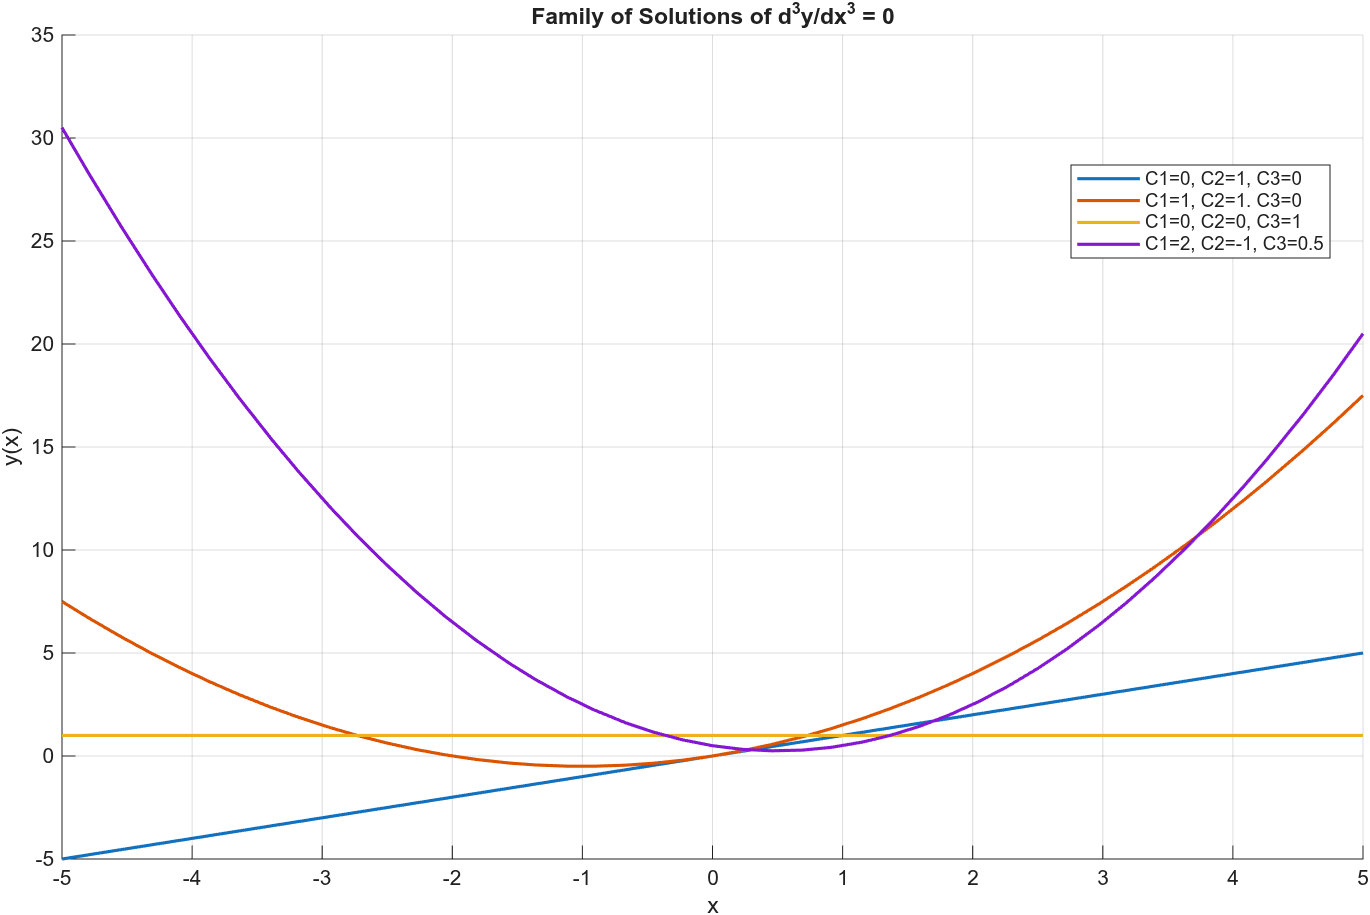
\includegraphics[width=0.7\textwidth]{Figure3.png}
\end{figure}

\end{document}
